\lab{Applications}{Weightloss and Predator-Prey Models}{Weightloss and Predator-Prey Models}
\label{lab:Weightloss}

\section{A Weightloss Model}
Here we will look at a model of weight change based on basic thermodynamics and kinematics.
The main idea behind weight change is simple.
If a person's energy intake is more than their energy expended, then they gain weight.
If their intake is less, then they lose weight.
Let the \emph{energy balance} $EB$ be the difference between \emph{energy intake} $EI$ and \emph{energy expenditure} $EE$, so that
\begin{equation}
\label{eqn:EB}
EB = EI - EE.
\end{equation}
When the energy intake is greater than the energy expended, the balance is positive and weight is gained.
Similarly, the balance is negative and weight is lost if the energy intake is less than the energy expended.

Body weight at time $t$ is the sum of the weight of fat and lean tissue; that is,  $BW(t) = F(t) + L(t).$
These quantities can be described by the compartmental model
\begin{subequations}
\label{eqn:compartment}
\begin{align}
\rho_F \dfrac{dF(t)}{dt} &= (1-p(t)) EB(t),\label{eqn:compartment:a}\\
\rho_L \dfrac{dL(t)}{dt} &= p(t) EB(t),\label{eqn:compartment:b}
\end{align}
\end{subequations}
where $p(t)$ and $1-p(t)$ represent the proportion of the energy balance ($EB(t)$) that results in a change in the quantity of lean or fatty tissue, respectively.
Constants $\rho_L$ and $\rho_F$ represent the energy density of lean and fatty tissue (about $1800$ and $9400$ kcal/kg).

Next we need to find expressions for $p(t)$ and $EB(t)$ in terms of $L$ and $F$ (the dependent variables), $PAL$ and $EI$ (possibly varying parameters), and other constant parameters.

 The proportion $p(t)$ will vary with $F$ and $L$; from Forbes' Law \cite{Fo.2} we have that
\begin{equation}
\label{eqn:forbes}
\dfrac{dF}{dL} = \dfrac{F}{10.4}.
\end{equation}
Hence,
\[
\dfrac{F}{10.4} = \dfrac{dF}{dL} = \dfrac{dF/dt}{dL/dt} = \dfrac{\dfrac{(1-p(t)) EB(t)}{\rho_F}}{\dfrac{p(t) EB(t)}{\rho_L}} = \dfrac{\rho_L}{\rho_F} \dfrac{1-p(t)}{p(t)}.
\]
Solving for $p(t)$ gives Forbes' equation
\begin{equation}
\label{eqn:Forbes2}
p(t) = \dfrac{C}{C+F(t)}\quad\mbox{where}\quad C=10.4\dfrac{\rho_L}{\rho_F}.
\end{equation}

We will use two expressions for energy expenditure (EE).
First, we have the formula
\begin{equation}
\label{eqn:EE0}
EE = PAL \times RMR,
\end{equation}
where $PAL$ is your physical activity level and $RMR$ your resting metabolic rate.
Your resting metabolic rate can be determined by using the Mifflin equation.
This equation is an estimate based on a population study and is widely used in the literature.
It takes into account your gender, age (A) in years, and height (H) in meters:
\begin{equation}
\label{eqn:RMR}
RMR = \begin{cases} 9.99 W + 625 H + 5 A + 5 & \mbox{if male}\\ 9.99 W + 625 H + 5 A -161 & \mbox{if female.}\end{cases}
\end{equation}  
Your physical activity level can be determined by using the table below.
\begin{table}[h]
\begin{center}
\begin{tabular}{|l|l|}
\hline
1.40--1.69 & People who are sedentary and do not exercise regularly, spend \\
& most of their time sitting, standing, with little body displacement
\\
\hline
1.70--1.99 & People who are active, with frequent body displacement throughout  \\
& the day or who exercise frequently\\
\hline
2.00--2.40 & People who engage regularly in strenuous work or exercise for \\
& several hours each day\\
\hline
\end{tabular}
\caption{This is a rough guide for physical activity level (PAL).  
% For more detailed estimates, see \cite{Heym} and Appendix \ref{PAL_appendix}.
}
\end{center}\label{tab:PAL_table}
\end{table}

The second expression for energy expenditure comes from decomposing more precisely the different ways that energy is expended:
\begin{equation}
\label{eqn:EE}
EE = \underbrace{\delta BW}_\text{\parbox{1cm}{physical\\activity}} + \underbrace{\beta_{tef} EI}_\text{\parbox{1cm}{thermic\\effect of\\eating}} + \underbrace{\beta_{at} EI + \gamma_F F + \gamma_L L + \eta_F \dfrac{dF}{dt} + \eta_L \dfrac{dL}{dt}  + K}_\text{resting metabolic rate (RMR)},
\end{equation}
where $\gamma_F = 22$ kcal/kg/d, $\gamma_L = 3.2$ kcal/kg/d, $\eta_F = 180$ kcal/kg, and $\eta_L = 230$ kcal/kg; see \cite{Hall.2, Hall.4}.
Further, we let $\beta_{tef}=0.10$ and $\beta_{at}=0.14$ denote the coefficients for the thermic effect of feeding and adaptive thermogenesis, respectively.
The parameter $\delta$ is the coefficient representing the amount of energy expended from physical activity per kilogram of body mass.
Notice that $\gamma_L$ is significantly larger than $\gamma_F$.
This means that lean tissue metabolizes energy much faster than fatty tissue.
As a result, there are instances where one may want to increase their lean body mass through resistance training so that they are better able to support a higher caloric intake without significant weight gain.
Finally, we remark that the constant $K$ can be tuned to an individual's body type directly through RMR and fat measurement, and is assumed to remain constant over time.

% Assumptions made/Areas to improve: 
% include more accurate approximation of PAL (given in appendix), BMI (show to vary with race), account for variation in body type.

Thus, since the input $EI$ is assumed to be known, we can use \eqref{eqn:EE} and \eqref{eqn:Forbes2} to write \eqref{eqn:compartment} in terms of $F$ and $L$, thus allowing us to close the system of ordinary differential equations (ODEs).

Specifically, we have
\begin{align*}
RMR(t) = \frac{EE}{PAL}&= K + \gamma_F F(t) + \gamma_L L(t) + \eta_F \dfrac{dF}{dt} + \eta_L \dfrac{dL}{dt}  + \beta_{at} EI\\
% &= K + \gamma_F F(t) + \gamma_L L(t) + \dfrac{\eta_F}{\rho_F} (1-p(t)) EB(t) + \dfrac{\eta_L}{\rho_L} p(t) EB(t)  + \beta_{at} EI,\\
\dfrac{1}{PAL}\left(EE - EI + EI \right) &= K + \gamma_F F(t) + \gamma_L L(t) \\
&+ \left(\dfrac{\eta_F}{\rho_F} (1-p(t)) + \dfrac{\eta_L}{\rho_L} p(t) \right) EB(t) + \beta_{at} EI.\\
\left(\dfrac{1}{PAL}-\beta_{at}\right) EI &= K + \gamma_F F(t) + \gamma_L L(t) \\
&+ \left(\dfrac{\eta_F}{\rho_F} (1-p(t)) + \dfrac{\eta_L}{\rho_L} p(t) + \dfrac{1}{PAL}\right) EB(t).
\end{align*}
% Thus,
% \[
% \left(\dfrac{1}{PAL}-\beta_{at}\right) EI = K + \gamma_F F(t) + \gamma_L L(t) + \left(\dfrac{\eta_F}{\rho_F} (1-p(t)) + \dfrac{\eta_L}{\rho_L} p(t) + \dfrac{1}{PAL}\right) EB(t).
% \]
Solving for $EB(t)$ in the last equation yields
\begin{equation}
\label{eqn:EB2}
EB(t) = \dfrac{\left( \dfrac{1}{PAL} - \beta_{at} \right) EI - K - \gamma_F F(t) - \gamma_L L(t)}{\dfrac{\eta_F}{\rho_F} (1-p(t)) + \dfrac{\eta_L}{\rho_L} p(t) + \dfrac{1}{PAL}}.
\end{equation}
% To find $K$, we note that
% \begin{equation}
% \label{eqn:K}
% K = \left(\dfrac{1}{PAL}-\beta_{at}\right) EI - \gamma_F F(t) - \gamma_L L(t) - \eta_F \dfrac{dF}{dt} - \eta_L \dfrac{dL}{dt}  - \dfrac{1}{PAL} EB.
% \end{equation}
In equilibrium ($EB = 0$), this gives us
\begin{equation}
\label{eqn:K2}
K = \left(\dfrac{1}{PAL}-\beta_{at}\right) EI - \gamma_F F - \gamma_L L.
\end{equation}
Thus, for a subject who has maintained the same weight for a while, one can determine $K$ by using \eqref{eqn:K2}, if they know their average caloric intake and amount of fat (assume $L=BW-F$).
The function \li{weight_odesystem} in the following code implements \eqref{eqn:compartment}.

\begin{lstlisting}
from math import log
# Fixed Constants:
rho_F       = 9400.
rho_L       = 1800.
gamma_F     = 3.2
gamma_L     = 22.
eta_F       = 180.
eta_L       = 230.
C           = 10.4  # Forbes constant
beta_AT     = 0.14  # Adaptive Thermogenesis
beta_TEF    = 0.1   # Thermic Effect of Feeding
K           = 0

def forbes(F):
    C1 = C * rho_L / rho_F
    return C1 / (C1 + F)

def energy_balance(F, L, EI, PAL):
    p = forbes(F)
    a1 = (1. / PAL - beta_AT) * EI - K - gamma_F * F - gamma_L * L
    a2 = (1 - p) * eta_F / rho_F + p * eta_L / rho_L + 1. / PAL
    return a1 / a2

def weight_odesystem(t, y, EI, PAL):
    F, L = y[0], y[1]
    p, EB = forbes(F), energy_balance(F, L, EI, PAL)
    return np.array([(1 - p) * EB / rho_F , p * EB / rho_L])

def fat_mass(BW, age, H, sex):
    BMI = BW / H**2.
    if sex == 'male':
        return BW * (-103.91 + 37.31 * log(BMI) + 0.14 * age) / 100
    else:
        return BW * (-102.01 + 39.96 * log(BMI) + 0.14 * age) / 100

\end{lstlisting}

\begin{problem}
Consider the initial value problem
\begin{subequations}
\label{eqn:weight_prob1}
\begin{align*}
\rho_F \dfrac{dF(t)}{dt} &= (1-p(t)) EB(t),\\
\rho_L \dfrac{dL(t)}{dt} &= p(t) EB(t),\\
F(0) &= F_0, \\
L(0) &= L_0.
\end{align*}
\end{subequations}
The ode is given above by the function \li{weight_odesystem}.
To solve this IVP for a specific individual we need initial conditions $F_0$ and $L_0.$
The function \li{fat_mass} given earlier calculates $F_0$ based on an individual's body weight (kg), age, height (meters), and gender.
$L_0$ is then given by $L_0 = BW - F_0$.

Suppose a 38 year old female, standing 5'8'' and weighing 160 lbs, reduces her intake from 
2143 to 2025 calories/day, and increases her physical activity from little to no exercise (PAL=1.4) to exercising to 2-3 days per week (PAL=1.5).  
Find and graph the solution curve for this single-stage weightloss intervention over a period of 5 years.

\end{problem}

\begin{problem}

Modify the preceding problem to handle a two stage weightloss intervention:
Suppose for the first 16 weeks intake is reduced from 2143 to 1600 calories/day and physical activity is increased from little to no exercise (PAL=1.4) to an hour of exercise 5 days per week (PAL=1.7).
The following 16 weeks intake is increased from 1600 to 2025 calories/day, and exercise is limited to only 2-3 days per week (PAL=1.5).

Find and graph the solution curve over a period of 32 weeks.
\end{problem}

\section{Two Predator-Prey Models}
The Lotka-Volterra predator-prey model is a well-known 
system of odes given by 
\begin{align*}
	\frac{du}{dt} &= au - buv,\\
	\frac{dv}{dt} &= -cv + duv.
\end{align*}
In these odes $u$ and $v$ represent the prey and predator populations, respectively. $a$ represents the rate of growth of the prey, and $bu$ the amount of prey being eaten.
Similarly, $c$ represents the rate of natural predator death, and $du$ the growth of the predatorpopulation due to the quantity of prey eaten.

Let us look at the dynamics of this system.
First we note that there are exactly two equilibria (fixed points): either $(u,v) = (0,0)$ corresponding to the extinction of both species, or $(u,v) = (\frac{c}{d},\frac{a}{b})$.
Furthermore, from the odes we can see that if $v=0$ (there is an absence of any predators) then the population of prey will grow exponentially.

To get a better idea of the dynamics of this system we will graph its phase portrait.
We begin by nondimensionalizing the system to reduce the number of parameters:
Let $U = \frac{d}{c}u,$ $V = \frac{b}{a}v$, $\bar{t} = at,$ and $\alpha = \frac{d}{a}$.
Substituting into the original odes we obtain the nondimensional system of equations
\begin{align*}
	\frac{dU}{d\bar{t}} &= U(1-V),\\
	\frac{dV}{d\bar{t}} &= \alpha V (U-1).
\end{align*}
In the following code we plot the phase portrait.
To plot the direction field for the equations we use \li{numpy}'s \li{meshgrid} function and \li{matplotlib}'s \li{quiver} function.

\begin{figure}[ht]
\centering
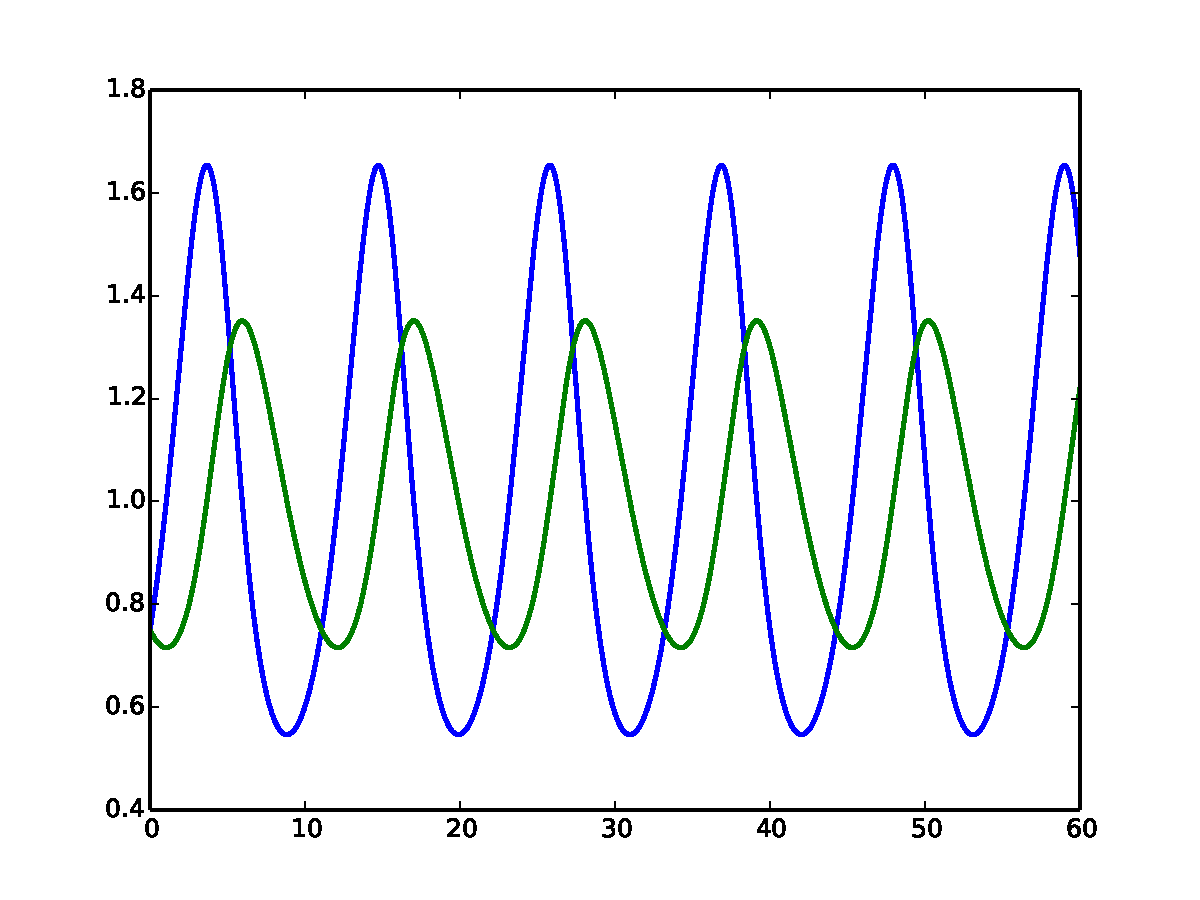
\includegraphics[width=\textwidth]{Lotka_Volterra.pdf}
\caption{The solution of the nondimensionalized Lotka-Volterra predator-prey equations with parameter $\alpha = 1/3$. 
This solution has initial conditions $(u,v) = (3/4, 3/4)$.}
\label{fig:pred-prey_Lotka_Voterra}
\end{figure}

\begin{lstlisting}
from scipy.integrate import odeint
a, b = 0., 13.                    # (Nondimensional) Time interval for one 'period'
alpha = 1. / 3                    # Nondimensional parameter
dim = 2                           # dimension of the system
y0 = np.array([1 / 2., 1 / 3.])   # initial conditions

# Note: swapping order of arguments to match the calling convention
# used in the built in IVP solver.
def Lotka_Volterra(y, x):
    return np.array([y[0] * (1. - y[1]), alpha * y[1] * (y[0] - 1.)])

subintervals = 200
# Using the built in ode solver
Y = odeint(Lotka_Volterra, y0, np.linspace(a, b, subintervals))

# Plot the direction field
Y1, Y2 = np.meshgrid(np.arange(0, 4.5, .2), np.arange(0, 4.5, .2), sparse=True, copy=False)
U, V = Lotka_Volterra((Y1, Y2), 0)
Q = plt.quiver(Y1[::3, ::3], Y2[::3, ::3],  U[::3, ::3],  V[::3, ::3], pivot='mid', color='b', units='dots',width=3.)
# Plot the 2 Equilibrium points
plt.plot(1, 1, 'ok', markersize=8)
plt.plot(0, 0, 'ok', markersize=8)
# Plot the solution in phase space
plt.plot(Y[:,0], Y[:,1], '-k', linewidth=2.0)
plt.plot(Y[::10,0], Y[::10,1], '*b')

plt.axis([-.5, 4.5, -.5, 4.5])
plt.title("Phase Portrait of the Lotka-Volterra Predator-Prey Model")
plt.xlabel('Prey',fontsize=15)
plt.ylabel('Predators',fontsize=15)
plt.show()
\end{lstlisting}

\begin{problem}
Compute the solutions $(u,v)$ of 
\begin{align*}
	\frac{dU}{d\bar{t}} &= U(1-V),\\
	\frac{dV}{d\bar{t}} &= \alpha V (U-1).
\end{align*}
for initial conditions $(1/2, 3/4)$, $(1/16, 3/4)$, and $(1/40, 3/4)$.
Add these solutions to the phase portrait of the Lotka-Volterra model.
Can you see any limitations of this model? 
\end{problem}

\begin{figure}[ht]
\centering
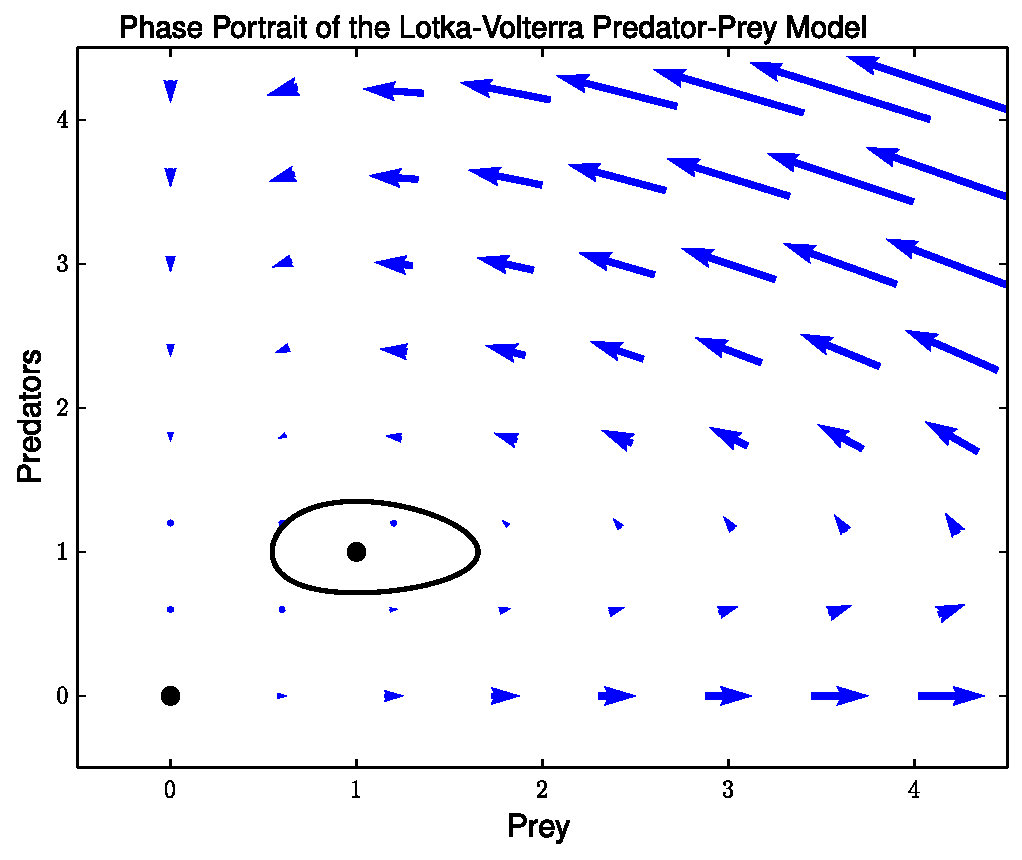
\includegraphics[width=\textwidth]{Lotka_Volterra_Phase_Portrait.pdf}
\caption{The phase portrait for the nondimensionalized Lotka-Volterra predator-prey equations with parameters $\alpha = 1/3$. 
The portrait includes the direction field, the two equilibrium points, and the graph of the solution with initial conditions $(u,v) = (3/4, 3/4)$. }
\label{fig:pred-prey_Lotka_Voterra_Phase_Portrait}
\end{figure}

We have already noticed that in the absence of predators, the Lotka-Volterra equations predict that the prey population will grow exponentially.
The logistic predator-prey equations change this dynamic by adding a term to give the prey population a carrying capacity $K$: 
\begin{align*}
	\frac{du}{dt} &= au\left(1 -\frac{u}{K}\right) - buv,\\
	\frac{dv}{dt} &= -cv + duv.
\end{align*}
Let $U = \frac{u}{K},$ $V = \frac{b}{a}v$, $\bar{t} = at,$  $\alpha = \frac{dK}{a}$, and $\beta = \frac{c}{dK}$.
Then the nondimensional logistic equations are 
\begin{align*}
	\frac{dU}{d\bar{t}} &= U(1-U-V),\\
	\frac{dV}{d\bar{t}} &= \alpha V (U-\beta).
\end{align*}

\begin{problem}
Compute the solutions $(u,v)$ of 
\begin{align*}
	\frac{dU}{d\bar{t}} &= U(1-U-V),\\
	\frac{dV}{d\bar{t}} &= \alpha V (U-\beta).
\end{align*}
for initial conditions $(1/3, 1/3)$ and $(1/2, 1/5)$.
Do this for parameter values $\alpha, \beta = 1, .3$ and also for values $\alpha, \beta = 1, 1.1$.
Create a phase portrait for the logistic equations using both sets of parameter values.
Remember to plot the direction field, all equilibrium points, and the orbits of the solutions.
\end{problem}